% !TeX root = ../main.tex
% CHU SO HUU: Minh Khoa và Ngọc Đô | KHONG THEO PREAMBLE, KHONG BEGIN DOCUMENT TRONG THAN PHAN NAY.
\section{Kết quả kiểm định Chi-square và mức độ liên hệ}
Giao thức TCP chứa $102\,689$ bản ghi, UDP chứa $14\,993$ bản ghi và ICMP chứa $8\,291$ bản ghi. Theo họ tấn công, nhóm Normal có $67\,343$ bản ghi, DoS có $45\,927$, Probe có $11\,656$, R2L có $995$ và U2R chỉ có $52$.
\begin{lstlisting}[firstnumber=1]
# Bảng chéo tần số quan sát
crosstab = pd.crosstab(df[col1], df[col2])
if order_col2:
    crosstab = crosstab.reindex(columns=[c for c in order_col2 if c in crosstab.columns])
print("\n[BẢNG CHÉO TẦN SỐ QUAN SÁT]")
print(crosstab)
\end{lstlisting}
Bảng~\ref{tab:t34:chi2-observed} trình bày bảng chéo tần số quan sát $O_{ij}$ của $n = 125\,973$ bản ghi theo \texttt{protocol\_type} và \texttt{attack\_category}.

\begin{table}[H]
  \centering
  \caption{Bảng chéo tần số quan sát $O_{ij}$ giữa \texttt{protocol\_type} và \texttt{attack\_category}}
  \label{tab:t34:chi2-observed}
  \begin{tabular}{lrrrrrr}
    \toprule
    & \multicolumn{5}{c}{\texttt{attack\_category}} & \\
    \cmidrule(lr){2-6}
    \texttt{protocol\_type} & DoS & Normal & Probe & R2L & U2R & Tổng \\
    \midrule
    ICMP & $2\,847$  & $1\,309$  & $4\,135$ & $0$   & $0$  & $8\,291$ \\
    TCP  & $42\,188$ & $53\,600$ & $5\,857$ & $995$ & $49$ & $102\,689$ \\
    UDP  & $892$     & $12\,434$ & $1\,664$ & $0$   & $3$  & $14\,993$ \\
    \midrule
    Tổng & $45\,927$ & $67\,343$ & $11\,656$ & $995$ & $52$ & $125\,973$ \\
    \bottomrule
  \end{tabular}
\end{table}

Tiếp theo, ta tính tần số kỳ vọng $E_{ij}$ cho $15$ ô của bảng và đối chiếu với quy tắc Cochran~\cite{task34_cochran1954}.
\begin{lstlisting}[firstnumber=1]
# Kiểm định Chi-square
chi2, p_value, dof, expected = stats.chi2_contingency(crosstab)

# Kiểm tra điều kiện kỳ vọng < 5
total_cells = expected.size
cells_under_5 = np.sum(expected < 5)
pct_under_5 = (cells_under_5 / total_cells) * 100
e_min = np.min(expected)
\end{lstlisting}
Chỉ một ô, cặp (ICMP, U2R), có $E_{ij} < 5$, tương ứng $6{,}7\%$ số ô, và giá trị kỳ vọng nhỏ nhất $E_{\min} = 3{,}42$ nằm ở chính ô này.\footnote{Tần số kỳ vọng $E_{ij}$ tỷ lệ thuận với tổng cột $C_j$. Tập NSL-KDD mất cân bằng nhãn nghiêm trọng, và nhóm U2R chỉ có $52$ quan sát, khoảng $0{,}04\%$ cỡ mẫu. Ở hàng ICMP, hàng nhỏ nhất với $8\,291$ bản ghi, ta có $E = 8\,291 \times 52 / 125\,973 = 3{,}42$. Mọi ô còn lại có $E_{ij} > 5$ vì các tổng hàng và tổng cột tương ứng đủ lớn.} Tỷ lệ vi phạm nhỏ hơn ngưỡng $20\%$, và $E_{\min}$ lớn hơn $0$ nên điều kiện kiểm định thỏa mãn. Ba ô có tần số quan sát bằng $0$ trong Bảng~\ref{tab:t34:chi2-observed} là (ICMP, R2L), (ICMP, U2R) và (UDP, R2L). Chúng không vi phạm điều kiện vì quy tắc Cochran xét tần số kỳ vọng, không xét tần số quan sát.

Kiểm định cho thống kê $\chi^2 = 25\,578{,}38$ với bậc tự do $df = (3 - 1)(5 - 1) = 8$ và $p\text{-value}$ tiệm cận $0$ (phần mềm hiển thị $0{,}0000\text{e}+00$).\footnote{Với $\chi^2 = 25\,578{,}38$ và $df = 8$, xác suất đuôi nhỏ hơn $10^{-5000}$, thấp hơn số thực dương nhỏ nhất mà kiểu số thực $64$ bit biểu diễn được. Thư viện làm tròn giá trị này về $0$.} Hệ số Cramér's $V$ tính theo công thức $V = \sqrt{\dfrac{\chi^2 }{\bigl(n \times \min(r - 1,\, c - 1)\bigr)}}$ đạt $V = 0{,}3186$.
\begin{lstlisting}[firstnumber=1]
# Tính Cramér's V
n = crosstab.to_numpy().sum()
min_dim = min(crosstab.shape) - 1
cramer_v = np.sqrt(chi2 / (n * min_dim))
\end{lstlisting}

Ta so sánh $p\text{-value}$ với mức ý nghĩa $\alpha = 0{,}05$. Vì $p\text{-value} \approx 0 < \alpha$, ta bác bỏ giả thuyết không $H_0$. Giao thức mạng và hình thức tấn công không độc lập với nhau: phân phối của \texttt{attack\_category} thay đổi theo \texttt{protocol\_type}. Cỡ mẫu $n = 125\,973$ đủ lớn để $p\text{-value}$ về $0$ với cả những liên hệ rất nhỏ, nên bằng chứng về độ mạnh của liên hệ nằm ở hệ số $V$.

Với $k = \min(r - 1,\, c - 1) = 2$, các mốc của $V$ trong Bảng~\ref{tab:t34:cramer-scale} là $0{,}07$ (nhỏ), $0{,}21$ (trung bình) và $0{,}35$ (lớn). Giá trị $V = 0{,}3186$ vượt mốc trung bình và nằm sát mốc lớn, thấp hơn $0{,}35$ khoảng $9\%$. Lưu lượng mạng chứa nhiều nhiễu: mỗi họ tấn công gồm nhiều kỹ thuật chạy trên nhiều dịch vụ, nên một đặc trưng đơn lẻ hiếm khi tách được các lớp. Một liên hệ ở mức này là tín hiệu có giá trị cho bài toán phân loại.

Để xác định các cặp giao thức và họ tấn công gây ra sự phụ thuộc, ta tính phần dư chuẩn hóa $Z_{ij} = \dfrac{O_{ij} - E_{ij}}{\sqrt{E_{ij}}}$ và biểu diễn chúng trên Hình~\ref{fig:chi2-heatmap}. Màu đỏ ứng với $Z_{ij} > 0$, tức cặp xuất hiện nhiều hơn mức kỳ vọng khi hai biến độc lập. Màu xanh ứng với $Z_{ij} < 0$, tức cặp xuất hiện ít hơn mức đó.
\begin{lstlisting}[firstnumber=1]
# Heatmap phần dư chuẩn hóa
residuals = (crosstab - expected) / np.sqrt(expected)
print("\n[PHẦN DƯ PEARSON CHUẨN HÓA Z_ij]")
print(residuals.round(2))
plt.figure(figsize=(10, 6))
sns.heatmap(
  residuals,
  annot=True,
  cmap="coolwarm",
  center=0,
  fmt=".1f",
  linewidths=0.5,
  cbar_kws={'label': 'Phần dư Pearson $Z_{ij}$'}
)
plt.title(f"Heatmap Phần dư chuẩn hóa: {col1.upper()} vs {col2.upper()}", fontsize=13, pad=12)
plt.xlabel(col2, fontsize=11)
plt.ylabel(col1, fontsize=11)
plt.tight_layout()
\end{lstlisting}

\begin{figure}[H]
  \centering
  \IfFileExists{figures/task34_heatmap_residuals_protocol_type.pdf}
  {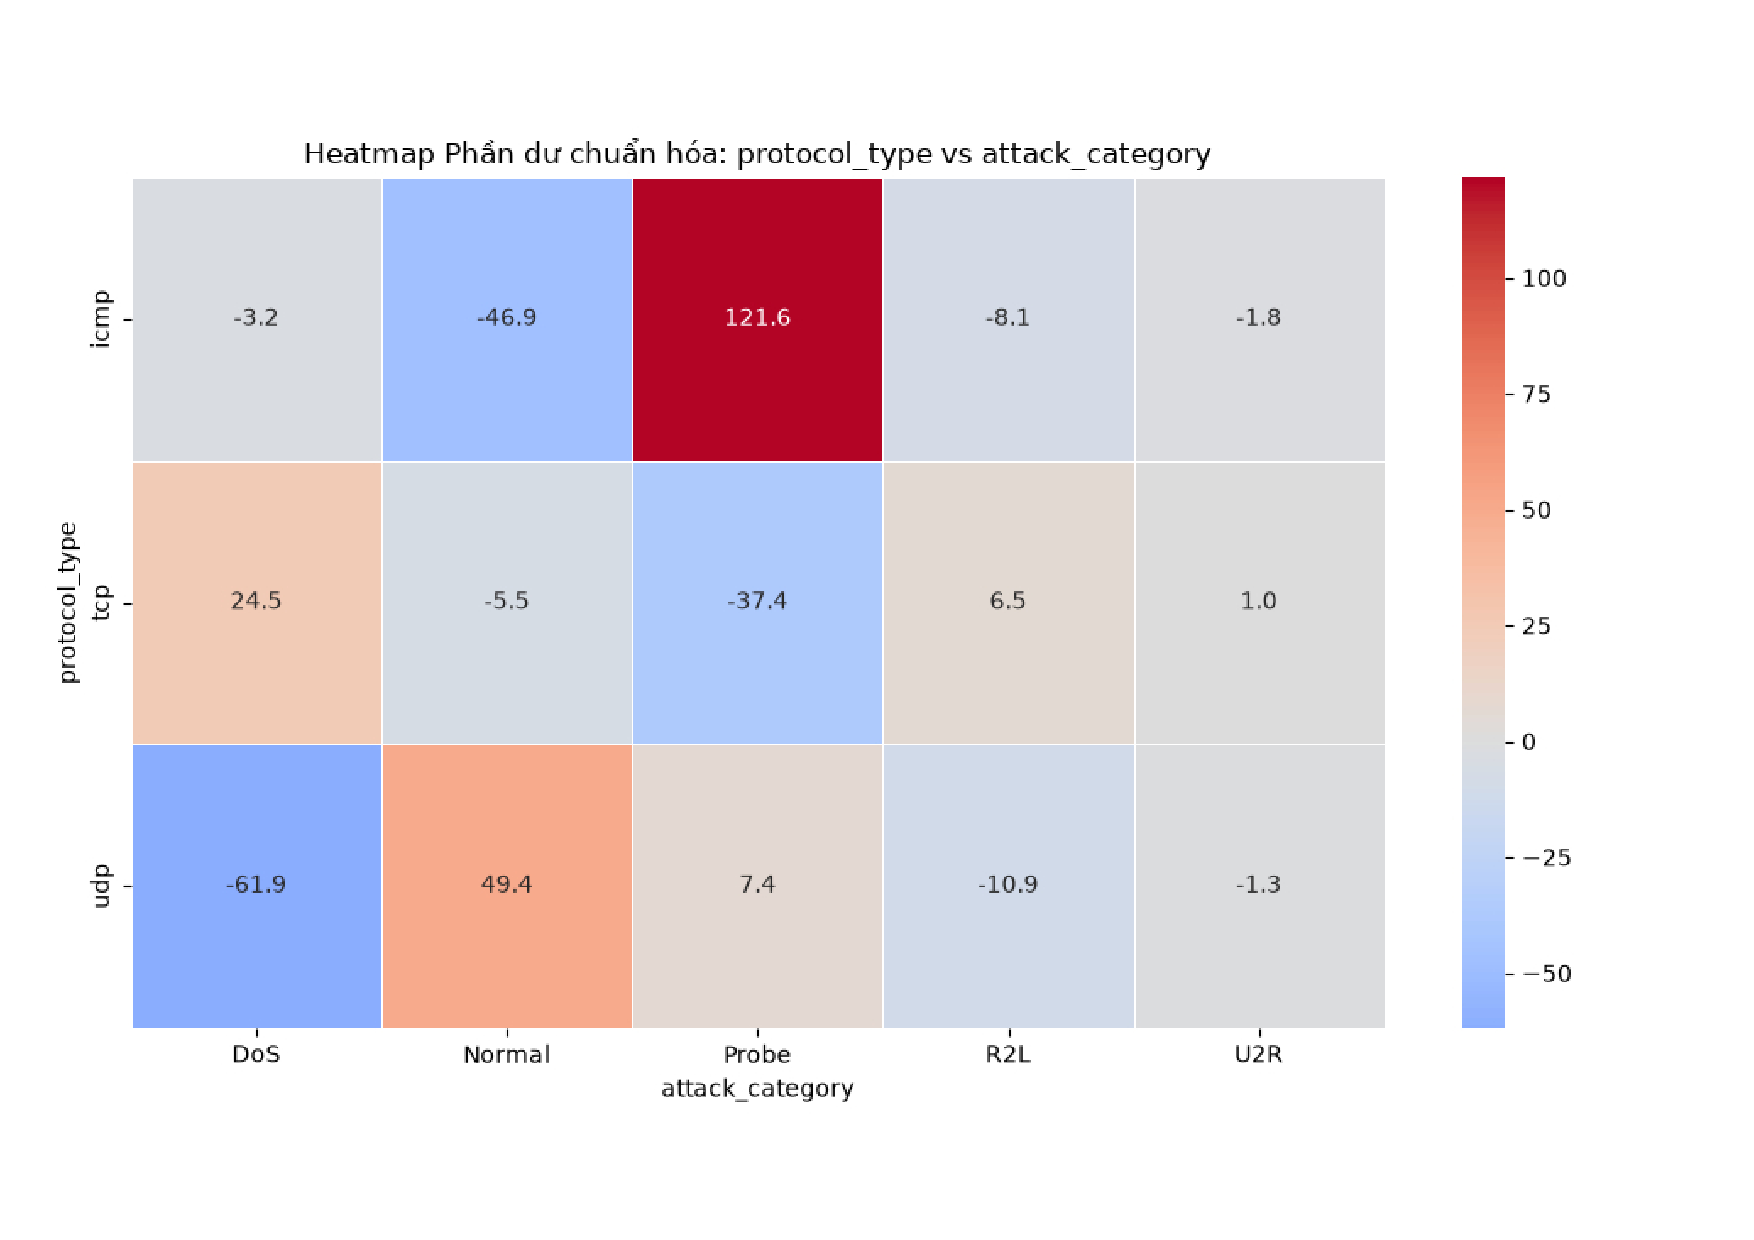
\includegraphics[width=0.9\textwidth]{task34_heatmap_residuals_protocol_type.pdf}}
  {\fbox{\parbox{0.8\textwidth}{\centering\vspace{3em}% [CHÈN ẢNH HEATMAP: đặt heatmap\_residuals.png vào thư mục figures/]
  \textcolor{red}{\textbf{[Chèn heatmap\_residuals.png]}}\vspace{3em}}}}
  \caption{Heatmap phần dư chuẩn hóa $Z_{ij}$ giữa \texttt{protocol\_type} và \texttt{attack\_category}}
  \label{fig:chi2-heatmap}
\end{figure}

Trong ma trận $Z_{ij}$, ba ô có $|Z|$ lớn nhất đều vượt ngưỡng $|Z| > 3$ từ $16$ lần trở lên. Ô đầu tiên là (ICMP, Probe) với $Z = +121{,}6$. Trong $8\,291$ bản ghi ICMP, $4\,135$ bản ghi thuộc nhóm Probe, tương đương $49{,}9\%$, trong khi Probe chỉ chiếm $9{,}3\%$ toàn mẫu. Số quan sát gấp khoảng $5{,}4$ lần số kỳ vọng ($767{,}15$). ICMP không mang dữ liệu ứng dụng và không dùng số hiệu cổng, nhưng cho phép gửi gói echo request đến cả dải địa chỉ để xác định máy nào đang hoạt động. Kẻ tấn công dùng đặc điểm này cho giai đoạn quét mạng và thăm dò, nên ICMP trong tập dữ liệu gắn với hoạt động do thám.

Ô thứ hai là (UDP, DoS) với $Z = -61{,}9$, phần dư âm có độ lớn đứng thứ hai. Chỉ $892$ bản ghi UDP thuộc nhóm DoS, thấp hơn nhiều so với $5\,466$ bản ghi kỳ vọng, và nhóm DoS chiếm $6{,}0\%$ lưu lượng UDP so với $36{,}5\%$ toàn mẫu. Kẻ tấn công từ chối dịch vụ trong tập dữ liệu né UDP và chọn TCP. TCP có cơ chế bắt tay ba bước và lưu trạng thái từng kết nối, nên một loạt gói SYN không hoàn tất bắt tay làm đầy bảng kết nối của máy chủ. UDP không có trạng thái kết nối để làm cạn tài nguyên theo cách đó. Dấu hiệu này cũng xuất hiện ở cặp (TCP, DoS) với $Z = +24{,}5$, một phần dư dương nhỏ hơn hai ô cực trị nhưng cùng chiều với cơ chế bão hòa tài nguyên.

Ô thứ ba là (UDP, Normal) với $Z = +49{,}4$. Có $12\,434$ bản ghi UDP thuộc nhóm Normal, nhiều hơn mức kỳ vọng $8\,015$, và nhóm Normal chiếm $82{,}9\%$ lưu lượng UDP so với $53{,}5\%$ toàn mẫu. UDP truyền tải chủ yếu các dịch vụ không hướng kết nối của người dùng hợp lệ, chẳng hạn truy vấn tên miền, và kẻ tấn công ít dùng giao thức này. Ba ô cực trị cho thấy mỗi giao thức mang một cấu hình lưu lượng riêng: ICMP nghiêng về thăm dò, TCP nghiêng về bão hòa tài nguyên, UDP nghiêng về lưu lượng bình thường.

Kết quả chỉ có giá trị trong phạm vi tập NSL-KDD. Tập dữ liệu này được tạo trong môi trường mô phỏng với tỷ lệ các họ tấn công do người xây dựng quyết định, nên các tỷ lệ trên không ước lượng được phân phối lưu lượng của mạng Internet thực tế, và ta không suy diễn kết quả ra ngoài phạm vi đó. Trong phạm vi tập dữ liệu, kẻ tấn công có xu hướng chọn lọc giao thức cụ thể cho từng phương thức xâm nhập. \texttt{protocol\_type} mang năng lực phân biệt cao giữa các họ tấn công, nên đặc trưng này cần giữ lại làm thuộc tính đầu vào cho các mô hình học máy phát hiện xâm nhập huấn luyện trên tập NSL-KDD.
